% Source: report/sections/04_results.md (owner: Manoj, #6).
\section{Results}
\label{sec:results}

\subsection{Main results}
\label{sec:main-results}
\Cref{tab:main} compares the five models on the same 120 test images. All numbers are means over images: each
image is scored on its own and then averaged, so a small polyp counts as much as a large one (\cref{sec:unet}).
``Dice @0.5'' uses the default probability threshold of 0.5. ``Dice tuned'' uses the threshold that was best on
the \textbf{validation} set (\cref{sec:threshold}). ``Dice TTA'' averages the predictions of four flipped views of each image
(test-time augmentation). The speed columns are explained in \cref{sec:speed}.

\begin{table*}[t]
  \centering
  \small
  \setlength{\tabcolsep}{5pt}
  \begin{adjustbox}{max width=\textwidth}
  \begin{tabular}{@{}lcccccccccc@{}}
    \toprule
    Model & Params (M) & Dice @0.5 & IoU @0.5 & Precision & Recall & Miss rate & Threshold & Dice tuned & Dice TTA & FPS (fp16) \\
    \midrule
    U-Net (scratch)     & 31.0         & 0.851          & 0.774          & 0.867          & 0.897          & 4.2\%          & 0.50 & 0.851          & 0.863          & 45.7 \\
    U-Net + ResNet-34   & 24.4         & 0.903          & 0.846          & 0.919          & 0.917          & 3.3\%          & 0.60 & 0.904          & 0.912          & \textbf{109.5} \\
    U-Net + MobileNetV2 & \textbf{6.6} & 0.894          & 0.835          & \textbf{0.928} & 0.898          & 5.0\%          & 0.45 & 0.894          & 0.900          & 91.7 \\
    Attention U-Net     & 31.4         & 0.854          & 0.775          & 0.868          & 0.895          & 5.0\%          & 0.55 & 0.854          & 0.857          & 40.7 \\
    SegFormer (MiT-B2)  & 24.7         & \textbf{0.917} & \textbf{0.865} & 0.911          & \textbf{0.943} & \textbf{2.5\%} & 0.60 & \textbf{0.918} & \textbf{0.926} & 43.3 \\
    \bottomrule
  \end{tabular}
  \end{adjustbox}
  \caption{Test results on Kvasir-SEG ($n = 120$). Best value per column in bold. ``Miss rate'' is the share of test images
  with Dice below 0.5, where the polyp was essentially not found. FPS is measured in fp16 for every model; SegFormer is
  the exception that runs faster in fp32 (56.9 frames per second, \cref{sec:speed}).}
  \label{tab:main}
\end{table*}

What the table shows:
\begin{itemize}
  \item \textbf{Baseline.} The U-Net trained from scratch already reaches a Dice of 0.851 and an IoU of 0.774. Its recall
        (0.897) is higher than its precision (0.867): it tends to over-segment a little, marking some healthy tissue
        around the polyp, rather than missing parts of the polyp.
  \item \textbf{Pretrained encoders.} Replacing the encoder with an ImageNet-pretrained CNN is the largest single
        improvement among the U-Nets: ResNet-34 reaches a Dice of 0.903 (+0.052 over the baseline) and MobileNetV2
        0.894 (+0.043), with fewer parameters (24.4\,M and 6.6\,M against 31.0\,M). With only 800 training images,
        features learned on ImageNet transfer well even though natural photographs look nothing like colonoscopy
        frames. ResNet-34 alone closes about four fifths of the gap between the baseline and SegFormer. The two
        encoders err in different directions: ResNet-34 is balanced (precision 0.919, recall 0.917), while MobileNetV2
        has the highest precision of all models (0.928) but a recall no better than the baseline's (0.898), so it
        tends to under-segment, leaving out parts of the polyp.
  \item \textbf{Attention gates.} The Attention U-Net differs from the baseline only by its four attention gates, and it
        scores almost the same: Dice 0.854 against 0.851, IoU 0.775 against 0.774. It misses 6 polyps instead of 5,
        and the gates (0.4\,M extra parameters, plus their extra computation at every skip connection) make it
        slightly slower (40.7 against 45.7 frames per second).
  \item \textbf{Transformer encoder.} SegFormer is the most accurate model: Dice 0.917 and IoU 0.865, 0.066 Dice above the
        baseline, with 6\,M fewer parameters. It has the highest recall (0.943) with a precision close to the best, so
        it finds more of each polyp without marking much extra tissue. It misses only 3 of the 120 polyps.
  \item \textbf{Threshold tuning.} The best validation thresholds ranged from 0.45 to 0.60, and tuning changed test Dice
        by at most 0.001 for every model (\cref{sec:threshold}). The predictions are sharp, with most pixels close to 0 or 1, so
        moving the threshold changes very few of them, and tuning is not a useful source of gain.
  \item \textbf{Test-time augmentation} raised the Dice of every model, by between 0.003 (Attention U-Net) and 0.012
        (baseline): ResNet-34 $0.903 \rightarrow 0.912$, MobileNetV2 $0.894 \rightarrow 0.900$, SegFormer $0.917 \rightarrow 0.926$. \Cref{sec:speed} discusses
        what it costs in speed.
\end{itemize}

\subsection{How certain are these numbers?}
\label{sec:ci}
120 test images are a sample: on another 120 polyps every mean would come out a little different. We estimate
how much with the \textbf{bootstrap}~\cite{efron1993bootstrap}: we draw 120 images from the test set \emph{with
replacement}, recompute the mean Dice, repeat this 2000 times and report the middle 95\% of these means as the
\textbf{95\% confidence interval} (CI).

To decide whether one model really beats another, we bootstrap the \textbf{per-image difference} in Dice between
the two models. Because both models are scored on the same images, an unusually easy or hard image affects both
equally, so this paired comparison is much more sensitive than comparing two separate intervals. A gain counts
as significant when its 95\% interval does not contain zero (two-sided $p < 0.05$).

\begin{table}[t]
  \centering
  \footnotesize
  \setlength{\tabcolsep}{2pt}
  \begin{adjustbox}{max width=\linewidth}
  \begin{tabular}{@{}lccc@{}}
    \toprule
    Model & Dice [CI] & Gain vs.\ baseline [CI] & $p$ \\
    \midrule
    U-Net (scratch)     & 0.851 [0.816, 0.883] & (baseline)                  &         \\
    U-Net + ResNet-34   & 0.903 [0.874, 0.928] & +0.052 [+0.028, +0.077]      & $<$0.001 \\
    U-Net + MobileNetV2 & 0.894 [0.862, 0.921] & +0.043 [+0.023, +0.065]      & $<$0.001 \\
    Attention U-Net     & 0.854 [0.822, 0.882] & +0.003 [$-$0.011, +0.018]    & 0.73    \\
    SegFormer (MiT-B2)  & 0.917 [0.893, 0.937] & +0.066 [+0.042, +0.093]      & $<$0.001 \\
    \bottomrule
  \end{tabular}
  \end{adjustbox}
  \caption{Mean test Dice with 95\% bootstrap CI, and the gain over the U-Net baseline (paired bootstrap, 95\% CI).}
  \label{tab:ci}
\end{table}

The baseline's interval is about $\pm0.034$ wide, so with 120 test images a single mean Dice is only known to within
about three hundredths. Even so, the paired comparison separates the models clearly (\cref{tab:ci}):
\begin{itemize}
  \item \textbf{Both pretrained CNNs and SegFormer beat the baseline significantly.} Their gain intervals lie entirely above
        zero; in none of the 2000 resamples was any of the three worse than the baseline.
  \item \textbf{The attention gates' gain is not significant.} The interval for the Attention U-Net's gain, $-0.011$ to
        $+0.018$, contains zero ($p = 0.73$): on this test set, the gates make no measurable difference.
\end{itemize}

Because three models are far above the baseline, the more useful question is whether they differ from each
other. \Cref{tab:pairwise} applies the same paired test to the three best models.

\begin{table}[t]
  \centering
  \small
  \begin{adjustbox}{max width=\linewidth}
  \begin{tabular}{@{}lcc@{}}
    \toprule
    Comparison & Dice gain [95\% CI] & $p$ \\
    \midrule
    SegFormer $-$ ResNet-34   & +0.014 [$-$0.006, +0.036] & 0.17  \\
    SegFormer $-$ MobileNetV2 & +0.023 [+0.008, +0.040]   & 0.005 \\
    ResNet-34 $-$ MobileNetV2 & +0.009 [$-$0.009, +0.027] & 0.33  \\
    \bottomrule
  \end{tabular}
  \end{adjustbox}
  \caption{Paired comparison between the three most accurate models.}
  \label{tab:pairwise}
\end{table}

SegFormer is significantly more accurate than MobileNetV2, but \textbf{not significantly more accurate than
ResNet-34}, and ResNet-34 is not significantly more accurate than MobileNetV2. ``Not significant'' does not mean
``the same'': these intervals are about $\pm0.02$ wide, so with 120 test images a real difference of 0.014 could
neither be confirmed nor ruled out. All pairs are in \texttt{results/summary/pairwise\_dice.csv}. These intervals
cover the choice of test images only, not the randomness of training (\cref{sec:limits}).

\subsection{Training curves}
\label{sec:curves}
\Cref{fig:curves} shows the training loss and the validation Dice of every model per
epoch. The two models trained from scratch learn slowly: the baseline reached its best validation Dice (0.855)
at epoch 54 of 60, the Attention U-Net (0.859) at epoch 47, and both needed about 39 epochs to come within 2\% of
their best. The three models with a pretrained encoder start much higher and converge in fewer epochs:
MobileNetV2 came within 2\% of its best after 16 epochs, ResNet-34 after 19 and SegFormer after only 8.
They peaked at validation Dice 0.894 (epoch 33 of 40), 0.899 (epoch 38) and 0.913 (epoch 23). Pretrained models
also trained much faster: 8 minutes for MobileNetV2, 9 for ResNet-34 and 12 for SegFormer, against 46 for the
baseline and 54 for the Attention U-Net. No model overfitted: the validation Dice at the last epoch was within
0.005 of each model's best.

\begin{figure*}[t]
  \centering
  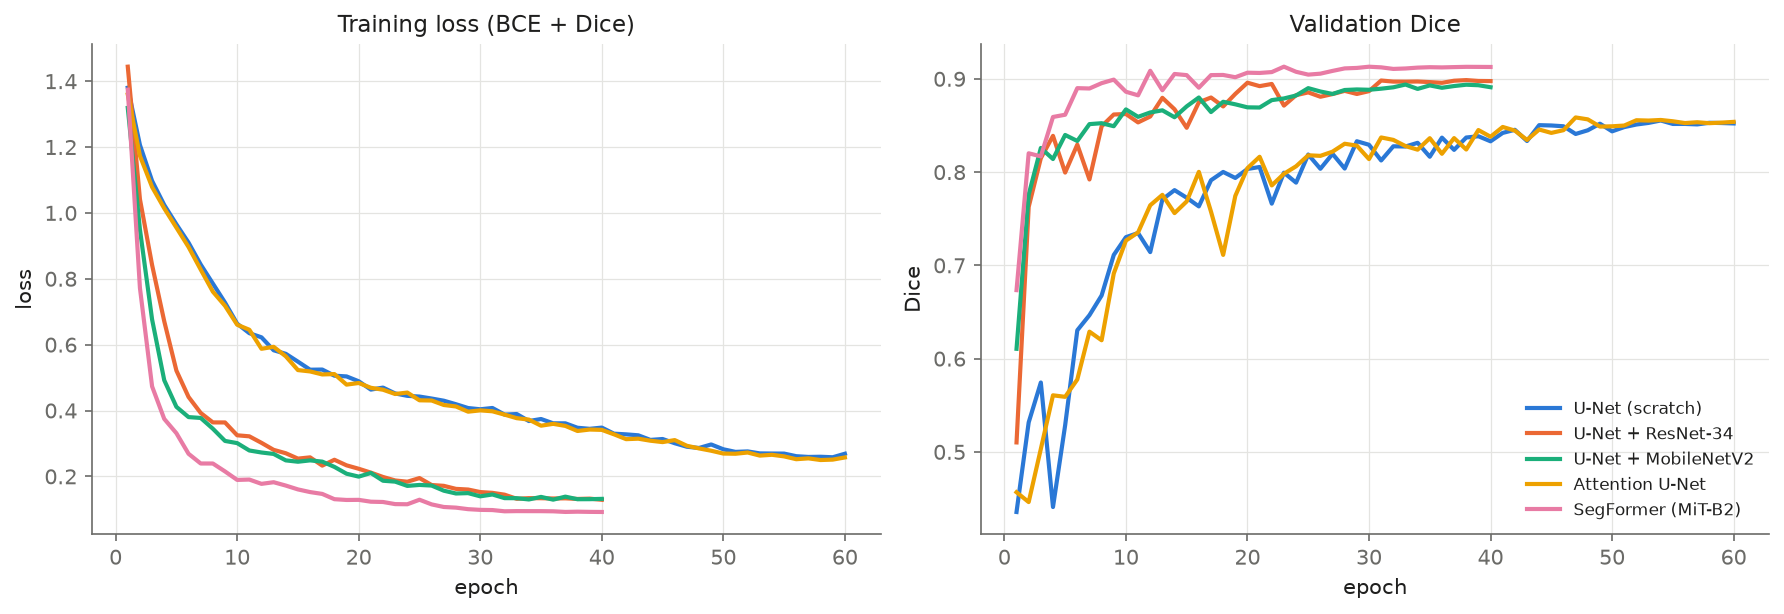
\includegraphics[width=0.92\textwidth]{training_curves.png}
  \caption{Training loss (left) and validation Dice (right) per epoch for all five models.}
  \label{fig:curves}
\end{figure*}

\subsection{Qualitative comparison}
\label{sec:quali}
\Cref{fig:comparison} shows five test polyps, from the smallest to the largest, with the
ground truth and the mask predicted by each model.
\begin{itemize}
  \item \textbf{The smallest polyp (0.5\% of the image)} separates the models most. The scratch U-Net and ResNet-34 both mark
        a large bright region nearby instead of the polyp (Dice 0.13 and 0.14). MobileNetV2 and the Attention U-Net find
        it only partly, among scattered false detections (0.50 and 0.59). Only SegFormer outlines it cleanly (0.82).
  \item \textbf{A thin, elongated polyp (5.5\%)}: the scratch U-Net breaks the mask into fragments (0.68), while the other four
        models score 0.91--0.96.
  \item \textbf{A medium polyp (11.7\%)} is easy for every model (all 0.96).
  \item \textbf{Large polyps (22.4\% and 71.9\%)}: the difference is in the quality of the mask. The two scratch models
        produce ragged, blocky borders, and on the largest polyp, which fills most of the frame, they leave holes and
        fragments (scratch U-Net 0.78, Attention U-Net 0.57). The three pretrained models produce smooth, filled masks
        (0.92--0.98).
\end{itemize}
Pretrained encoders therefore help at both ends of the size range: they find small polyps more often and give
cleaner, complete masks on large ones.

\begin{figure*}[t]
  \centering
  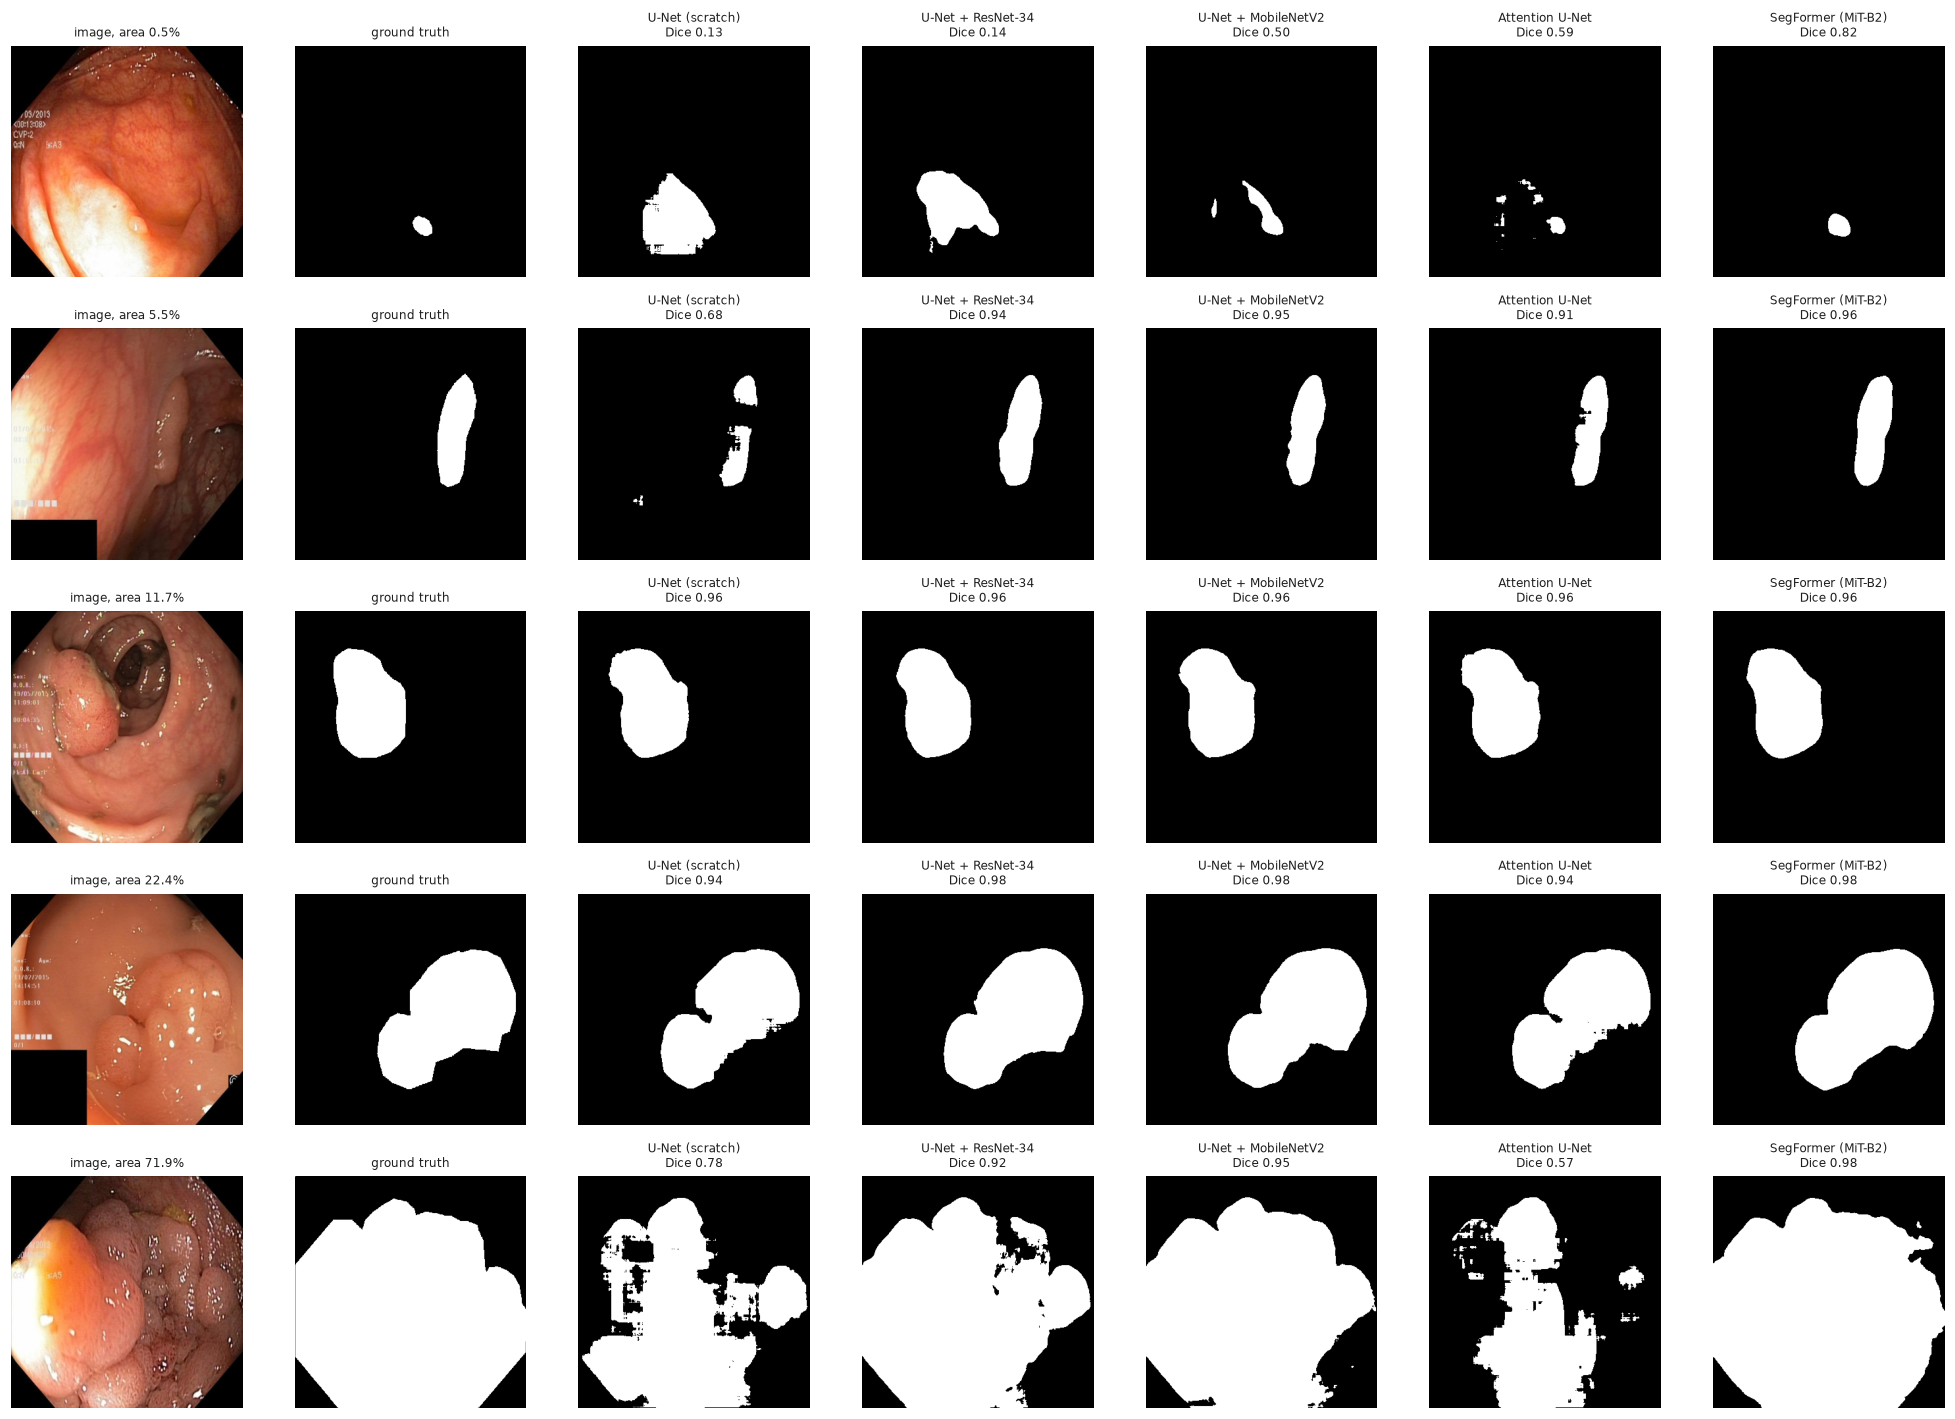
\includegraphics[width=0.86\textwidth]{model_comparison.png}
  \caption{Five test polyps, from the smallest to the largest: image, ground truth and the mask predicted by each model, with its Dice.}
  \label{fig:comparison}
\end{figure*}

\subsection{Summary}
\label{sec:results-summary}
The five models fall into three accuracy tiers. The two U-Nets trained from scratch score about 0.85, and
attention gates add nothing measurable. The U-Nets with ImageNet-pretrained CNN encoders reach 0.89--0.90, a
significant gain from transfer learning alone. SegFormer, with a pretrained transformer encoder, is the most
accurate at 0.917, although its lead over ResNet-34 is not statistically significant on 120 test images. All
five models run above 25 frames per second in fp16. \Cref{fig:accspeed} puts accuracy
and speed together: U-Net + ResNet-34 gives the best accuracy for its speed, as the fastest model (109.5 frames
per second) and within the error margin of SegFormer. \Cref{sec:failure} shows where the remaining errors are.

\begin{figure}[t]
  \centering
  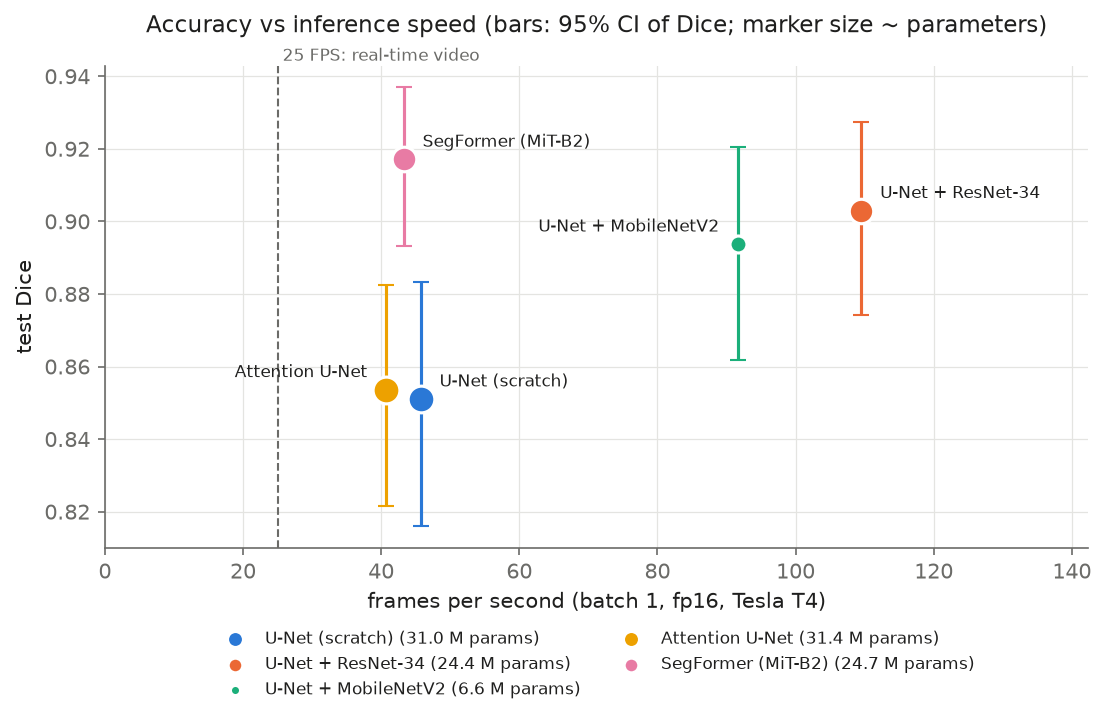
\includegraphics[width=\linewidth]{accuracy_vs_speed.png}
  \caption{Test Dice against inference speed (batch 1, fp16, T4 GPU). Vertical bars: 95\% bootstrap confidence interval of the Dice; marker size grows with the number of parameters; dashed line: 25 frames per second.}
  \label{fig:accspeed}
\end{figure}
